\subsection{Aprendizaje de Máquina}
\subsubsection{Definición}
El Aprendizaje de Máquina (ML) según \textcite{Ethem2014} no solo está relacionado con los conjuntos de datos, sino que es una parte integra de la Inteligencia Artificial, es decir, es la construcción de una aproximación a partir de datos históricos que puede llegar a suministrar salidas correctas. \textcite{Bost2015} Menciona que el Aprendizaje de Máquina se utiliza para diferentes tareas tales como detección de correo basura, reconocimiento facial y estimaciones financieras, pero de igual forma se utiliza en otras áreas como robótica y medicina, es decir, no está ligada a un solo campo del saber.

La aplicación de métodos Aprendizaje de Máquina a bases de datos se le conoce como Minería de Datos, puesto que la extracción de las materias primas extraídas en esos sitios son procesados con el fin de producir material más refinado. Este material refinado son los datos de entrada de todo modelo de Inteligencia Artificial, ya sea Aprendizaje de Máquina o Aprendizaje Profundo. Pero en vista de que esos datos representan una parte importante para la generación de modelos, es necesario garantizar la integridad y seguridad de esa información, debido a que pueden contener información sensible de una organización o personas.

\subsubsection{Tipos de problemas}
Los tipos de problemas en Aprendizaje de Máquina se clasifican en tres grupos dependiendo del tipo de entrada y salida requerida. Según autores como \textcite{Russell2003, Han2012, raschka2015python} estos grupos son: Aprendizaje Supervisado, no Supervisado y Reforzado.

\paragraph{Aprendizaje Supervisado} Este tipo de aprendizaje es sinónimo de clasificación. El Aprendizaje Supervisado aporta como principal herramienta algoritmos con el fin de clasificar información etiquetada a partir de datos históricos. Por lo tanto, a partir de la información conocida se puede predecir los datos a futuro, ya sea un grupo, una cantidad numérica o una clase binaria.

Este tipo de algoritmo es el principal utilizado en el presente proyecto, no solo porque permite realizar gran parte de las tareas que todo estudiante en sus primeros años de formación académica necesita, sino que a diferencia de los demás, este es el que mayormente se utiliza en los cursos iniciales de ciencias de datos, mientras que los demás son de uso más avanzado.

\paragraph{Aprendizaje no Supervisado} Este tipo de aprendizaje es sinónimo de Agrupamiento. El proceso de aprendizaje se considera no supervisado dado que las entradas son datos no etiquetados. Debido a que no se ingresan datos etiquetados al algoritmo de aprendizaje, es el propio algoritmo que se encarga de clasificar los resultados. El Aprendizaje no Supervisado puede traer problemas como tener que descubrir los patrones ocultos en la información, pero sin importar ese inconveniente, puede ser la mejor elección para generar un modelo de Inteligencia Artificial.

\paragraph{Aprendizaje Reforzado} En este caso el modelo intenta tomar acciones viables para maximizar la recompensa en una situación en particular. Es aplicado por varios software como videojuegos para encontrar el mejor camino posible o comportamiento que se debería tomar en una situación especifica. El entrenamiento reforzado se diferencia del supervisado, dado que los datos de entrenamiento tienen sus respectivas predicciones o respuestas, mientras en el reforzado el modelo se entrena sin datos, es decir, decide que acciones realizar para cumplir con la tarea suministrada con base a la experiencia que acaba de obtener.

\subsubsection{Tipos de predicción}
La ruta general en Aprendizaje de Máquina Supervisado consiste en una serie de pasos que inicia con la obtención del conjunto de datos y termina con las métricas del modelo entrenado y probado. Conforme a lo mencionado por \textcite{oswald2020python} en su libro ``\textit{Python 3 for Machine Learning}'' estos pasos son:

\begin{APAenumerate}
    \item Obtener el conjunto de datos.
    \item Limpiar el conjunto de datos.
    \item Seleccionar las característica y reducir la dimensionalidad.
    \item Seleccionar algoritmo de Aprendizaje de Máquina.
    \item Separar el conjunto de datos en entrenamiento y pruebas.
    \item Entrenar el modelo.
    \item Probar el modelo.
    \item Optimizar el modelo y obtener el rendimiento.
\end{APAenumerate}

Independientemente del proceso necesario para obtener las predicciones utilizando Aprendizaje de Máquina Supervisado, es necesario elegir el tipo de predicción que se va a realizar, seleccionar el modelo más óptimo para el conjunto de datos, ajustar los hiperparámetros y si es necesario reducir la dimensionalidad. Cada uno de los tipos de predicción tiene sus propios algoritmos basados en estadística y matemática, que de acuerdo con \textcite{Geron2019,oswald2020python} son Clasificación, Regresión y Agrupamiento, pero por simplicidad se consideran en este proyecto como cajas negras.

\paragraph{Clasificación} La salida obtenida es del tipo Booleano, es decir, uno, cero, verdadero, falso, si o no. La clasificación (ver Figura ~\ref{fig:ejclasi}) en pocas palabras es asignar nuevas entradas al modelo para generar la predicción más probable con base a la clase, pero si hay un desbalance significativo entre las posibles salidas, lo más seguro es que el resultado no sea correcto.

 \begin{figure}[H]
    \centering
    \caption{Ejemplo de Clasificación}
    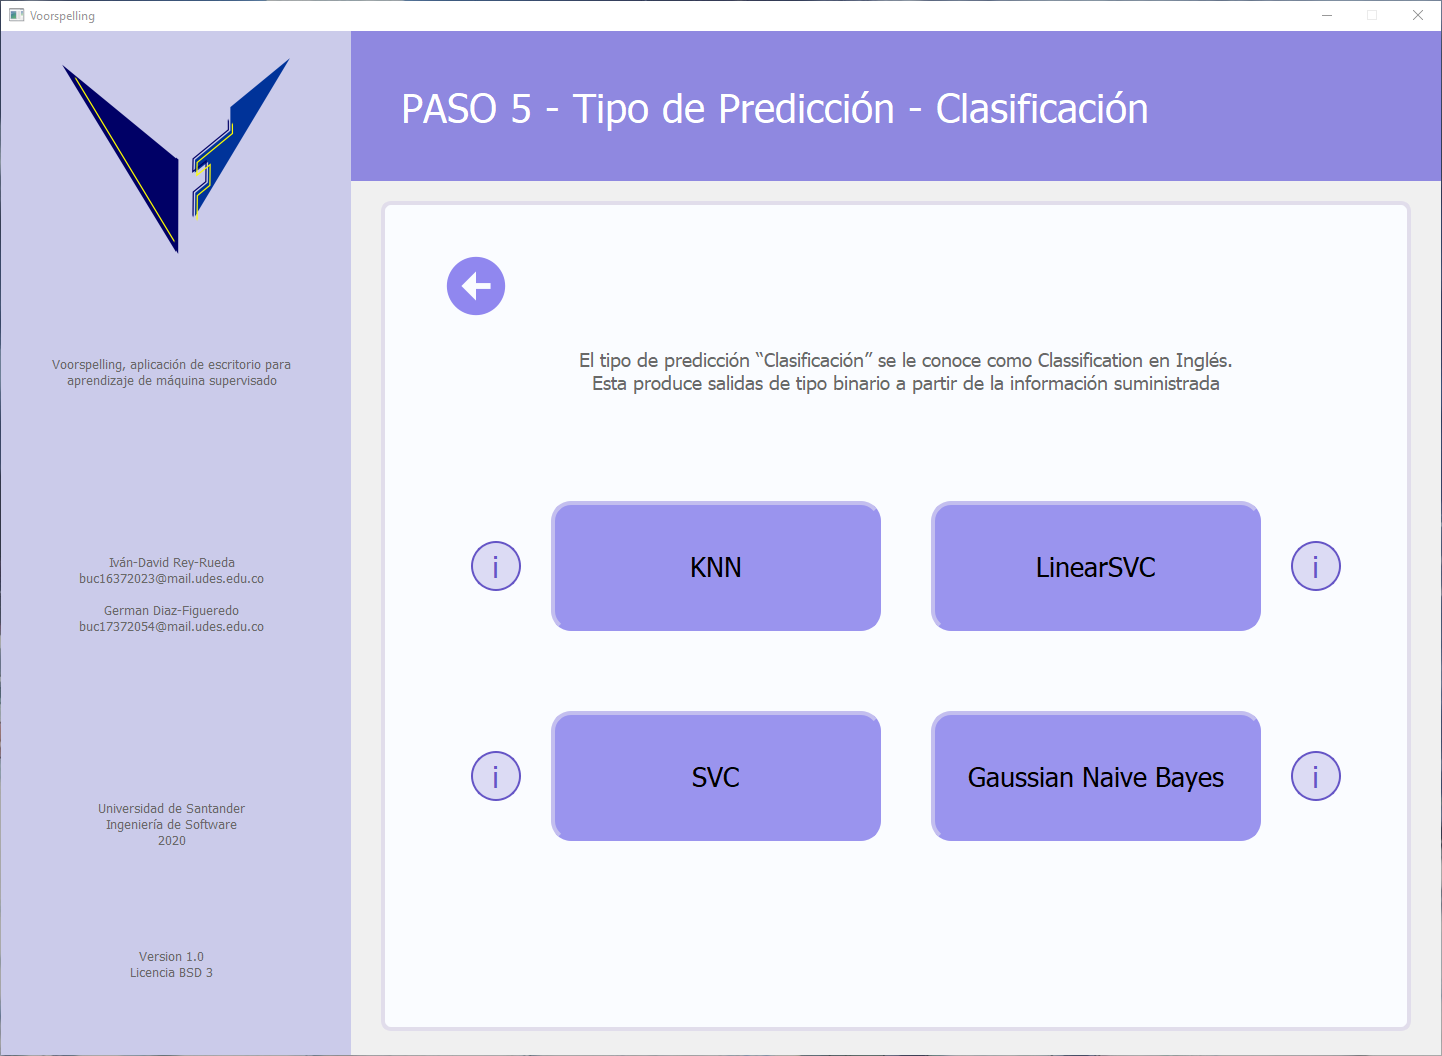
\includegraphics[trim=0 0 0 25, scale=0.54]{classification}
    \caption*{Nota\normalfont. La recta de color verde representa el plano que separa los datos, entre aquellos que son verdadero con valor uno y falso con valor cero.}
    \vskip-4ex
    \label{fig:ejclasi}
\end{figure}

Este tipo de clasificación se utiliza para predecir una clase discreta o etiqueta que puede tener dos estados, pero si el problema lo requiere se puede utilizar clasificación multi-clase. La clasificación con múltiples clases a diferencia de la clasificación binaria, no tiene únicamente los estados esperado y no esperado, sino que las salidas son clasificadas en una de todas las clases disponibles. 

Los modelos disponibles para Clasificación en Python a través de la librería scikit-learn \parencite{sklearn_api} que se utilizan en este proyecto son:

\begin{APAitemize}
    \item SVC rbf: La implementación de este estimador esta basada en libsvm con kernel igual a \textit{rbf}. El tiempo de entrenamiento se incrementa hasta el orden cuadrático cuando el número de muestras supera las diez mil unidades, por lo tanto es recomendable usar otras opciones si se presenta tal situación.
    \item LinearSVC: Similar a SVC con kernel igual a \textit{linear}, pero implementado en términos de liblinear en vez de lbsvm, por ende adquiere más flexibilidad en la selección de penalizaciones y pérdidas de función, con lo que tiene la posibilidad de escalar mejor para grandes cantidades de muestras.
    \item KNN: \textit{K Nearest Neighbours} Es un algoritmo que almacena los casos disponibles y realiza la clasificación de nuevos casos apoyándose en una medición de similaridad con base a la distancia \textit{k} entre una muestra y la otra.
    \item Gaussian Naive Bayes: Este estimador hace parte de los métodos Naive Bayes. Estos algoritmos están basados en la implementación de teorema de Bayes con la suposición de una independencia condicional entre las características, y de igual forma el algoritmo de clasificación Naive Bayes Gaussiana supone que la probabilidad de las características es Gaussiana.
\end{APAitemize}

\paragraph{Regresión} En este tipo de predicción el resultado se calcula a partir de un modelo que minimice la función de pérdida. Dado que la salida de estos algoritmos es un número, la Regresión (ver Figura ~\ref{fig:ejregre}) puede ser empleada tanto en problemas para clasificar clases, como estimar cantidad numéricas. Por tal motivo, es utilizada para predecir todo tipo de situaciones donde la salida sean datos continuos, por ejemplo: el valor de un seguro de vida y el valor en bolsa. 

\begin{figure}[H]
    \centering
    \caption{Ejemplo de Regresión}
    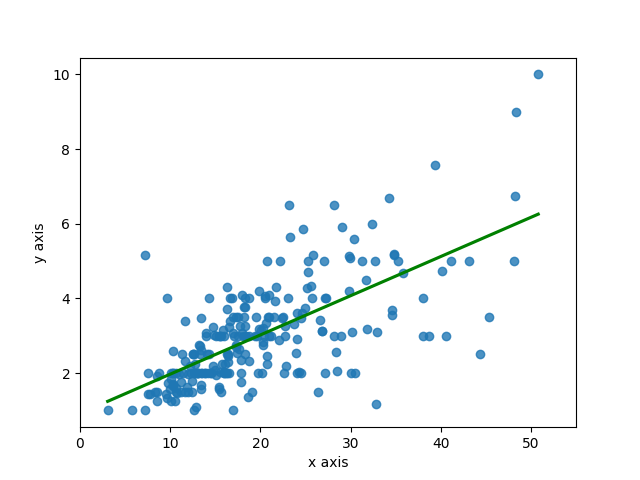
\includegraphics[trim=0 0 0 25,scale=0.5]{regression}
    \caption*{Nota\normalfont. La recta de color verde representa el comportamiento medio de los datos a partir de la función $f(x) = m\cdot x+b$ donde \textit{m} es la pendiente y \textit{b} el punto de corte con la abscisa.}
    \vskip-4ex
    \label{fig:ejregre}
\end{figure}

Los modelos disponibles de Regresión en Python a través de la librería scikit-learn \parencite{sklearn_api} que se utilizan en este proyecto son:

\begin{APAitemize}
    \item Lasso: Es un tipo de regresión lineal que utiliza contracción de los valores con base a un punto central, al igual que la media. Este procedimiento fomenta modelos más simples y dispersos, lo que que se traduce a modelos con menos parámetros.
    \item SGDClassifer: Este estimador implementa modelos lineales regulados, con un gradiente aleatorio de aprendizaje en descenso. El gradiente de las pérdidas se estima en cada muestra a la vez que modelo se actualiza en paraleo con la curva de aprendizaje.
    \item SVR rbf: Los parámetros en el modelo son \textit{C} y \textit{epsilon}. La implementación es basada en libsvm con kernel igual a \textit{rbf}. El tiempo de entrenamiento supera el orden cuadrático, de manera que es difícil trabajar con este modelo cuando el número de muestras supera las diez mil unidades.
    \item LinearSVR: Similar a SVC con kernel igual a \textit{linear}, pero implementado en términos de liblinear en vez de lbsvm. Permite mayor flexibilidad en la selección de penalizaciones y perdidas de función, y además escala mejor para grandes cantidades de muestras.
\end{APAitemize}

\paragraph{Agrupamiento} A este tipo de algoritmos se les conocen en inglés como \textit{Clustering} (ver Figura ~\ref{fig:ejcluster}). Su principal objetivo es entrenar un algoritmo para generar las agrupaciones deseadas, dado un conjunto de datos con sus respectivos datos históricos. La similitud de los grupos está dada por información adicional suministrada por el usuario, lo que puede convertirse en un problema de optimización de hiperparámetros, sobre todo si hay muchos atributos que deben considerarse para el entrenamiento. 

\begin{figure}[H]
    \centering
    \caption{Ejemplo de Agrupamiento}
    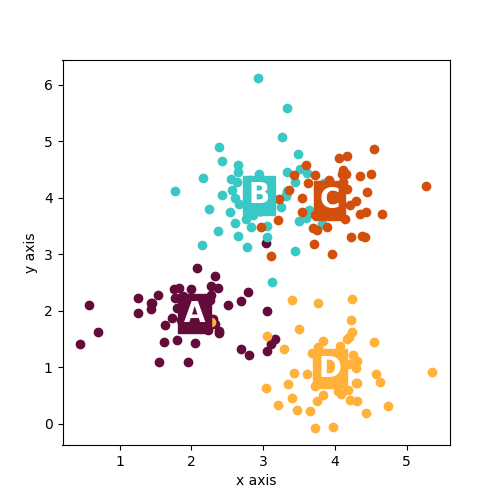
\includegraphics[trim=0 0 0 25,scale=0.5]{cluster}
    \caption*{Nota\normalfont. Cada \textit{cluster} está separado según su color. En este ejemplo, los grupos que se quieren predecir son A, B, C y D.}
    \vskip-4ex
    \label{fig:ejcluster}
\end{figure}

Los modelos disponibles de Agrupamiento en Python a través de la librería scikit-learn \parencite{sklearn_api} que se utilizan en este proyecto son:

\begin{APAitemize}
    \item Spectral Clustering: El agrupamiento espectral se utiliza cuando la estructura de agrupamiento es altamente no convexa, o mejor dicho cuando la medida del centro y la propagación del grupo no son viables para la descripción del grupo. Este modelo cuando llama al método entrenar, crea una matriz de afinidad usando una función kernel como \textit{rbf} o una matriz de conectividad de los \textit{k} vecinos más cercanos, dependiendo de los parámetros iniciales establecidos.
    \item Kmeans: Este algoritmo agrupa información tratando de separar muestras en un numero de grupos equivalente a la varianza, minimizando un criterio conocido como la inercia o suma de los cuadrados dentro de un grupo. Este algoritmo requiere un número de grupos especificados desde el inicio, pero trabaja bien para un gran número de muestras, a diferencia de otros modelos.
    \item Minibatch Kmeans: Este algoritmo es una variante del algoritmo KMeans, el cual utiliza minilotes para reducir el tiempo de compilación, mientras optimiza la función objetivo.
    \item Meanshift: Esta forma de agrupamiento tiene como fin descubrir irregularidades en una superficie de muestras. Este algoritmo está basado en datos centrales llamados centroides, los cuales funcionan convirtiendo los candidatos a centroides en la media de los puntos dentro de una determinada región. Estos candidatos son filtrados en una etapa de post-procesamiento con la finalidad de eliminar cualquier duplicado cercanos del conjunto de centroides finales.
\end{APAitemize}

\subsubsection{Selección de hiperparámetros}
\textcite{Wu2019} en su artículo \enquote{\textit{Hyperparameter optimization for machine learning models based on Bayesian optimization}} mencionan que los hiperparámetros son de gran importancia en el Aprendizaje de Máquina, dado que se encargan de cambiar el comportamiento de los algoritmos cuando entrenan el modelo. Por lo tanto, los hiperparámetros tienen una relación directa en el rendimiento final de cualquier modelo de Aprendizaje de Máquina, y no deben ser establecidos en valores arbitrarios, sino que se deben ser valores obtenidos de algoritmos tales como búsqueda Exhaustiva o Bayesiana.

\paragraph{Búsqueda exhaustiva} Este tipo de búsqueda es conocida como en inglés como \textit{greedy}. La búsqueda Exhaustiva implica realizar una exploración utilizando todos los valores posibles dada una lista de elementos $S$, pero en la mayoría de casos no se busca optimizar un solo hiperparámetro, sino que se requiere realizar una búsqueda para al menos dos o más listas de valores. Esto da como resultado tiempos de ejecución polinómicos, es decir $O(n^k)$ donde \textit{k} es el número de listas de valores o espacios de parámetros y \textit{n} la cantidad de elementos en el espacio $S$, si todos las listas tienen la misma longitud.

Este algoritmo se encuentra disponible en la librería scikit-learn \parencite{sklearn_api} para Python, con dos diferentes opciones: GridSearchCV y RandomSearchCV. La opción elegida para este proyecto es GridSearchCV (ver Figura ~\ref{fig:impbusexh}), dado que esta puede realizar una búsqueda exhaustiva con todo el espacio de valores, a diferencia de RandomSearchCV que escoge un subconjunto del espacio de valores con respecto a una semilla aleatoria.

\begin{figure}[H]
    \centering
    \caption{Implementación de Búsqueda Exhaustiva}
    \inputminted{Python}{pycode/gridsearch.py}
    \label{fig:impbusexh}
\end{figure}

\paragraph{Búsqueda Bayesiana}  Este algoritmo está basado en el teorema de Bayes y se le conoce como búsqueda Bayesiana. A diferencia de una búsqueda Exhaustiva, es una de las estrategias más eficientes con respecto al número de evaluaciones necesarias. Esta búsqueda es utilizada comúnmente cuando las ya mencionadas evaluaciones requieren de grandes cantidades de tiempo, cuando el problema no es convexo y cuando no se tiene una expresión para la función objetivo, pero si se puede obtener la información de los eventos de la función \parencite{Brochu2010}. 

Este algoritmo se encuentra disponible en la librería scikit-learn \parencite{sklearn_api} para Python con el nombre de BayesSearchCV (ver Figura ~\ref{fig:impbusbay}), y aunque existan otras opciones de vanguardia, utilizar directamente la implementación de scikit-learn beneficia al proyecto en el tiempo de desarrollo requerido para desplegar la aplicación.

\begin{figure}[H]
    \centering
    \caption{Implementación de Búsqueda Bayesiana}
    \inputminted{Python}{pycode/bayesiansearch.py}
    \label{fig:impbusbay}
\end{figure}


\subsubsection{Reducción de dimensionalidad}
Existe la creencia respecto al volumen de los datos que más información es mejor, y por lo general es cierto, pero no en todos los casos esto se cumple. Un mayor número de observaciones redunda en un mejor modelo, pero un mayor número de variables no necesariamente lo hace mejor \parencite{Guerrero2016}. Para conjuntos de datos con varias dimensiones, la reducción de dimensionalidad se ejecuta antes de aplicar los algoritmos de Aprendizaje de Máquina, con el propósito de evitar los problemas relacionados a la maldición de la dimensionalidad. Por tales motivos, autores en años anteriores como \textcite{Finley2005} mencionan que la selección de características se convierte en la opción mas viable, especialmente en conjuntos de datos con alta dimensionalidad.

Existen diferentes tipos de métodos con los cuales se aborda el problema de la reducción de la dimensionalidad, sin embargo, de acuerdo con \textcite{Finley2005,Sanchez-Marono2007} los más utilizados son los métodos de filtrado y envolventes. Estos métodos pretenden hallar un subconjunto de datos a partir del original, es decir, que el nuevo subconjunto candidato a ser la opción óptima pierde una o más características en el proceso. Esto da como resultado en el mejor de los casos un incremento en el rendimiento del clasificador, mientras que por otro lado, si el proceso de selección de características no es necesario desde el inicio, el resultado final es un clasificador con un rendimiento menor al inicial, dado que las características eliminadas eran significativas. 
 
\paragraph{Métodos de filtrado} Los métodos de filtrado realizan un análisis de las características individuales para identificar su importancia relativa. Son computacionalmente eficaces e independientes del modelo, pero por otro lado, es posible que una característica no sea útil por si sola, aunque puede ser significativa cuando está asociada con otra. Esta situación representa una desventaja en los métodos de filtrado, ya que se puede perder la potencial importancia de dichas características. 

Los algoritmos disponibles para métodos de filtrado en Python a través de la librería scikit-learn \parencite{sklearn_api} son:
 
 \begin{APAitemize}
     \item VarianceThreshold: es un método para la selección de características que remueve toda aquella característica cuya varianza no supere cierto límite. Adicionalmente, por defecto elimina toda característica con varianza cero, es decir aquellas que tienen el mismo valor en todas las muestras y por ende no otorgan información relevante.
     \item SelectKBest: este algoritmo se encarga de remover todas las características que no pertenezcan a las \textit{k} de características con mayor peso. La salida puede ser un nuevo vector con las nuevas características o el peso individual de cada una de ellas.
     \item SelectPercentile: es un algoritmo que remueve toda característica que el usuario no seleccione entre las de mayor puntuación.
     \item GenericUnivariateSelect: este algoritmo utiliza una estrategia configurable para realizar una selección de características univariadas.
 \end{APAitemize}
 
\paragraph{Métodos envolventes} Este tipo de métodos inician el proceso de evaluación de las características una a una, para luego seleccionar aquella que tiene el mejor rendimiento. Una vez terminado ese proceso se realiza la selección de las posibles combinaciones hasta que el modelo no tenga un mejor rendimiento con respecto a la última iteración. 
 
Los algoritmos disponibles para métodos envolventes en Python a través de la librería scikit-learn \parencite{sklearn_api} son:
 
 \begin{APAitemize}
     \item Recursive Feature Elimination: El objetivo de este método es la eliminación de características generando un conjunto de características cada vez más pequeño. Las características menos importantes son eliminadas del conjunto de características actuales, proceso que se repite constantemente hasta llegar a la cantidad requerida de características
     \item SelectFromModel: Este algoritmo puede ser utilizado con cualquier estimador que tenga los atributos coeficiente o importancia de característica, después de realizar el entrenamiento del modelo. Las características por defecto son consideradas no relevantes al no superar el umbral suministrado, mientras que aquellas que califican como importantes se mantienen.
     \item Sequential Feature Selector: Es un algoritmo exhaustivo que se utiliza para reducir el espacio de características de cierta dimensionalidad a un espacio de menor dimensionalidad. Tiene como finalidad seleccionar automáticamente un subconjunto de características que son relevantes para el problema. 
     \item Exhaustive Feature Selector: Este algoritmo evalúa subconjuntos de características exhaustivamente aplicando todas las posibles combinaciones. El mejor subconjunto se selecciona a partir del rendimiento obtenido entre todas las iteraciones con el modelo seleccionado, ya sea Regresión o Clasificación.
 \end{APAitemize}
 
\subsubsection{Aprendizaje automático}
Inicialmente todos los procesos de Aprendizaje de Máquina se realizaban paso a paso, pero con el desarrollo del primer algoritmo automatizado por parte de \textcite{Thornton2013} en su trabajo titulado ``\textit{Auto-Weka}'' el panorama cambia a uno donde es más efectivo utilizar algoritmos de aprendizaje automático para problemas de nivel empresarial. La ruta más fácil para seleccionar un estimador utilizada por estudiantes es definida a partir de la popularidad que tenga o que tan sencillo parece de utilizar, por consiguiente no se consideran las alternativas disponibles que pueden ser más eficientes. Parte de esos inconvenientes son remediados con los repositorios de acceso libre desarrollados para el uso de la comunidad, tales como: Weka \parencite{Hall2009}, scikit-learn \parencite{scikit-learn} y mljar-supervised \parencite{mljar2018}, los cuales ofrecen paquetes de selección de características, hiperparámetros y modelo por medio de sus algoritmos de aprendizaje automático.

En trabajos posteriores \textcite{Feurer2020} en su artículo ``\textit{Auto-Sklearn 2.0: The Next Generation}'' mencionan que a partir de mejoras en su algoritmo original de Auto-sklearn, obtienen mejoras significativas a partir de la implementación de una técnica de meta-aprendizaje más sencilla, la cual según los autores es el futuro para tener un Aprendizaje de Máquina automatizado cercano a la perfección y que además sea de libre acceso. No obstante, implementar esta librería actualmente no es posible dado que aún se encuentra en desarrollo, y pese a que la versión 1.0 se encuentra disponible desde el año 2016, es únicamente para sistemas operativos Linux. Por tales motivos, la librería utilizada para cubrir las funcionalidades de aprendizaje automático en el presente proyecto es mljar-supervised (ver Figura ~\ref{fig:impautoml}), la cual es desarrollada por \textcite{mljar2018} como un proyecto de software libre. Esta librería al igual que otros algoritmos de aprendizaje automatizado, tiene las funcionalidades de vanguardia necesarias para ejecutar optimización de hiperparámetros y selección de modelo, dado que si es necesario, los usuarios de \textit{Voorspelling} pueden elegir entre un proceso paso a paso o automático; decisión que está relacionada al objetivo del proyecto.

\begin{figure}[H]
    \centering
    \caption{Implementación de AutoML}
    \inputminted{Python}{pycode/automl.py}
    \label{fig:impautoml}
\end{figure}
